\documentclass[tikz,border=3mm]{standalone}
\usepackage[siunitx]{circuitikz}
\usetikzlibrary{calc,positioning,arrows.meta}

\begin{document}

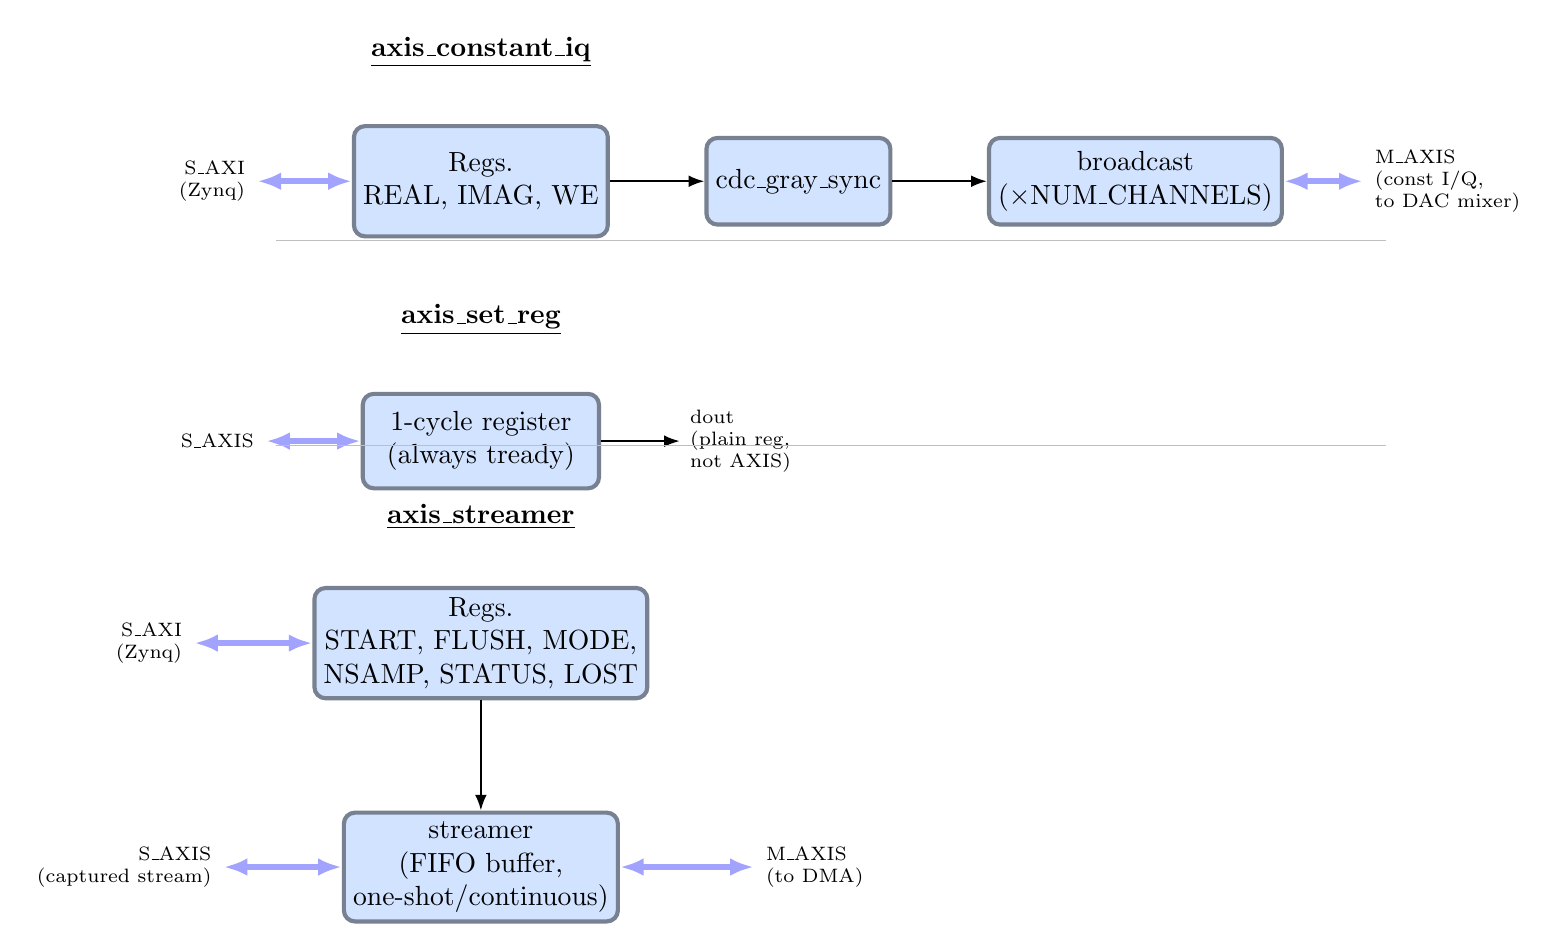
\begin{tikzpicture}
[box/.style={align=center, draw,rounded corners,minimum width=1.9cm,minimum height=1.1cm,draw={rgb,255:red,120; green,129; blue,145},fill={rgb,255:red,210; green,227; blue,255},line width=1.5pt},
titlestyle/.style={font=\bfseries},
arrow/.style={line width=2.2pt,draw={rgb,255:red,162; green,163; blue,255},{Latex[length=3mm]}-{Latex[length=3mm]}},
single arrow/.style={line width=0.8pt,-{Latex[length=2mm]}},
node distance=0.5cm]

% ---- axis_constant_iq ----
\node[titlestyle] (t1) at (0,0) {\underline{axis\_constant\_iq}};
\node[box,below=0.6cm of t1,minimum height=1.4cm] (ciq regs) {Regs.\\REAL, IMAG, WE};
\node[box,right=1.2cm of ciq regs] (ciq sync) {cdc\_gray\_sync};
\node[box,right=1.2cm of ciq sync,minimum width=2cm] (ciq bcast) {broadcast\\($\times$NUM\_CHANNELS)};
\draw[arrow] ($(ciq regs.west)+(-1.2,0)$) node[anchor=east,font=\scriptsize,align=right] {S\_AXI\\(Zynq)} -- (ciq regs.west);
\draw[single arrow] (ciq regs.east) -- (ciq sync.west);
\draw[single arrow] (ciq sync.east) -- (ciq bcast.west);
\draw[arrow] (ciq bcast.east) -- ++(1,0) node[anchor=west,font=\scriptsize,align=left] {M\_AXIS\\(const I/Q,\\ to DAC mixer)};

% ---- separator ----
\draw[gray!50,thin] (-2.6,-2.4) -- (11.5,-2.4);

% ---- axis_set_reg ----
\coordinate (row2) at (0,-3.4);
\node[titlestyle] (t2) at (row2) {\underline{axis\_set\_reg}};
\node[box,below=0.6cm of t2,minimum height=1.2cm,minimum width=3cm] (setreg) {1-cycle register\\(always tready)};
\draw[arrow] ($(setreg.west)+(-1.2,0)$) node[anchor=east,font=\scriptsize,align=right] {S\_AXIS} -- (setreg.west);
\draw[single arrow] (setreg.east) -- ++(1,0) node[anchor=west,font=\scriptsize,align=left] {dout\\(plain reg,\\ not AXIS)};

% ---- separator ----
\draw[gray!50,thin] (-2.6,-5.0) -- (11.5,-5.0);

% ---- axis_streamer ----
\coordinate (row3) at (0,-5.9);
\node[titlestyle] (t3) at (row3) {\underline{axis\_streamer}};
\node[box,below=0.6cm of t3,minimum height=1.4cm] (str regs) {Regs.\\START, FLUSH, MODE,\\NSAMP, STATUS, LOST};
\node[box,below=1.4cm of str regs,minimum width=2.4cm] (streamer) {streamer\\(FIFO buffer,\\ one-shot/continuous)};
\draw[arrow] ($(streamer.west)+(-1.5,0)$) node[anchor=east,font=\scriptsize,align=right] {S\_AXIS\\(captured stream)} -- (streamer.west);
\draw[single arrow] (str regs.south) -- (streamer.north);
\draw[arrow] ($(str regs.west)+(-1.5,0)$) node[anchor=east,font=\scriptsize,align=right] {S\_AXI\\(Zynq)} -- (str regs.west);
\draw[arrow] (streamer.east) -- ++(1.7,0) node[anchor=west,font=\scriptsize,align=left] {M\_AXIS\\(to DMA)};

\end{tikzpicture}

\end{document}
